% Created 2022-05-14 sáb 14:10
% Intended LaTeX compiler: pdflatex
\documentclass[11pt]{article}
\usepackage[utf8]{inputenc}
\usepackage[T1]{fontenc}
\usepackage{graphicx}
\usepackage{longtable}
\usepackage{wrapfig}
\usepackage{rotating}
\usepackage[normalem]{ulem}
\usepackage{amsmath}
\usepackage{amssymb}
\usepackage{capt-of}
\usepackage{hyperref}
\usepackage{geometry}
\geometry{ a4paper, total={170mm,257mm},left=20mm, top=35mm, bottom=35mm, right=20mm}
\usepackage{multicol}
\author{Ieremies Romero (217938)}
\date{}
\title{MO824 - Atividade GRASP}
\hypersetup{
 pdfauthor={Ieremies Romero (217938)},
 pdftitle={MO824 - Atividade GRASP},
 pdfkeywords={},
 pdfsubject={},
 pdfcreator={Emacs 28.1 (Org mode 9.6)},
 pdflang={Portuguese}}
\usepackage{biblatex}
\addbibresource{bib.bib}
\begin{document}

\maketitle
\section*{Descrição do problema}
\label{sec:orgaca3795}
\subsection*{Modelo matemático}
\label{sec:org4c9a73c}
A partir do problema da \emph{Maximum Quadratic Binary Function} (MAX-QBF), proposto por \cite{qbf},  o problema de maximização da função \(f: \mathbb{B}^{|x|} \to \mathbb{R}\), onde \(|x|\) é a dimensão do problema, descrita como
\[f(x_{1},\dots, f(x_{n})) = \sum \limits_{i=1}^{n} \sum \limits_{j=1}^{n} a_{i,j} x_{i} x_{j} ,\]
 em que \(a_{i,j} \in \mathbb{R} (i,j = 1,\dots,n)\) são os coeficientes da função.

A este problema adicionamos a restrição
\[ \sum_{i=1}^{n} w_{i} x_{i} \leq W ,\]
onde \(w_{i}\) é dito o peso da variável \(x_{i}\). Nosso objetivo nessa nova versão chamada \emph{Maximum Knapsack Quadratic Binary Function} (MAX-KQBF) é maximizar a função, tal que a soma dos pesos das variáveis na solução não exceda \(W\).

Nesse problema, nossas variáveis de decisão consistem em tornar ou não um certo \(x_{i}\) para valor \(1\) ou não. Isso será representado no código como inserir ou não na solução.

Durante esse relatório, nos referiremos a \(c(x_{i})\) como o custo que o elemento \(x_{i}\) incumbe a atual solução. Caso \(x_{i}\) já esteja na solução, ele é a diferença no valor da função objetivo da solução atual e sem ele. Caso \(x_{i}\) não pertença à solução, \(c(x_{i})\) é a diferença no valor da função objetivo da solução atual e com ele.
\section*{Metodologia}
\label{sec:orgb4cff69}
Para esse problema utilizaremos a meta-heurística \textbf{GRASP} (\emph{greedy randomized adaptive search procedure}), proposta por \cite{resende19_grasp} para problemas de minimização. Esta consiste em alternamos entre duas fases: uma fase construtiva e outra de busca local. Na primeira, utilizamos uma heurística gulosa aleatória para construir uma solução. Se esta não for viável, concertemo-na, tornando-a uma solução viável. Na segunda, realizamos uma busca local partindo desta solução. Por fim, repetimos esse processo um certo número de vezes, guardando a melhor solução encontrada.

É importante salientar que, como demonstrado em \cite{rezende19_grasp}, não é necessário fazer a etapa de "reparo" da solução se só incluirmos nela aqueles que não irão torná-la inviável. Tais variáveis são chamadas \textbf{candidatas} e, a cada iteração da etapa de construção, montamos (ou atualizamos) a chamada lista de candidatas \textbf{CL}.

Nesta etapa, a cada iteração analisamos cada elemento da lista CL e qual custo que sua inserção na solução irá causar. Em posse do maior e menor custos nesta lista, selecionamos aleatoriamente elementos que estão suficientemente próximos do menor custo, tais elementos compõem a chamada \textbf{lista restrita de candidatas} (RCL). A definição de suficientemente fica a cargo do parâmetro \textbf{\(\alpha\)} e é relativa ao intervalo de valores que obtivemos na análise da lista. Podemos repetir esse processo até que a lista de candidatos seja esgotada.

Já na etapa de busca local, analisamos as vizinhanças da nossa solução procurando por melhorias locais até não ser mais possível. Para cada problema, podem existir diversas definições de vizinhança e mais de um podem ser utilizadas nessa fase.

\subsection*{Heurística construtiva}
\label{sec:orge28a9ab}
Neste projeto, utilizamos como heurística padrão, um algoritmo muito similar ao proposto por \cite{rezende19_grasp}.

Iniciamos com uma lista de candidatos CL composta por todos os elementos podem ser adicionados a solução e que, se o feito, infringirão na restrição de peso. A cada interação, atualizamos CL com o mesmo critério, removendo aqueles que não podem mais serem adicionados.

Baseado no custo adicional que cada candidata incumbirá à solução quando inserida, determinamos quais os maiores (\(maxCost\)) e menores (\(minCost\)) custos e, baseado no parâmetro \(\alpha\), determinamos a lista de candidatos restritos de forma gulosa por
\[ RCL = \{ cand : c(cand) \leq minCost + \alpha \ (maxCost - minCost) \}. \]

Por fim, concluímos a interação da heurística realizando o passo aleatório: escolhemos um elemento de RCL aleatoriamente a ser inserido na nossa solução. Observe que o parâmetro \(\alpha\) determina o espaço amostral que teremos para retirar nosso elemento aleatório. Caso este seja pequeno de mais, realizamos apenas uma heurística gulosa, caso seja grande de mais, temos um algoritmo extremamente aleatório. Nesse experimento trabalhamos com dois valores de \(\alpha\): \(\alpha_{1} = 0.05\) e \(\alpha_{2} = 0.17\).

Para a heurística construtiva, consideramos como critério de parada quando a nossa lista de candidatas CL se tornar vazia ou nenhuma inserção que possamos fazer irá melhorar nossa função objetivo.

\subsection*{Métodos construtivos alternativos}
\label{sec:org49def5d}
Algumas alterações nesse método construtivo padrão são apresentadas em \cite{rezende19_grasp}. Dentre elas, aplicamos \textbf{random plus greedy} e \textbf{POP}.

\subsubsection*{Random plus greedy}
\label{sec:orgaf8c61c}
Nessa variante para a heurística construtiva, ao invés de tomarmos decisões gulosas e depois aplicarmos a aleatoriedade, fazemos o inverso. A partir da lista CL, retiramos uma amostra aleatória de tamanho máximo \(p\) para compor nossa RCL. Dentro da RCL, escolhemos o elemento com menor custo.

Nesse experimento, inicialmente tratamos \(p =0.5|x|\), mas, como será observado na seção \hyperref[sec:org01ea080]{Resultados}, outros valores também foram posteriormente testados.

\subsubsection*{POP}
\label{sec:org8f1cac4}
\emph{Proximate Optimality Principle} (POP) baseia-se na ideia de que "boas soluções são encontradas perto de outras boas soluções". Assim, nessa variante, realizamos buscas locais em certos momentos da heurística construtiva. No nosso caso, sabemos que a heurística irá tomar no máximo \(|CL|\) do \(CL\) inicial e, usando essa estimativa, realizamos uma busca local depois de \(33\%\) e \(66\%\) das iterações terem sido realizadas.
\subsection*{Busca local}
\label{sec:orgff5d321}
Na etapa de busca local, como descrito anteriormente, partimos de uma solução viável e, analisando a(s) vizinhança(s) desta solução, tomamos "passos" em direção a melhorar nossa função objetivo. O desafio então jaz em decidir quem serão nossas vizinhanças já que qualidade da busca depende diretamente nelas.

As vizinhanças a serem utilizadas são \(3\), compostas pelas soluções viáveis que diferem da atual pela:
\begin{itemize}
\item inserção de um novo elemento da CL na solução.
\item remoção de um elemento já presente solução.
\item substituição de um elemento na solução por outro na CL.
\end{itemize}

É importante ressaltar que a cada passo, a lista CL é atualizada com os elementos que não infringirão a restrição de peso, garantindo que a busca local sempre irá permanecer com soluções viáveis.

Uma vez que as vizinhanças estão definidas, é importante determinar qual dos passos será tomado. Duas abordagens são estudadas nesse experimento: \textbf{best-improving} e \textbf{first-improving}. Na primeira, percorremos todos os vizinhos (definidos pelas vizinhanças acima) e tomamos o passo na direção do vizinho que melhor afeta nossa função objetivo (no caso nosso caso, o de maior contribuição). Em contrapartida, a segunda nos propõe a tomar o primeiro "bom vizinho", ou seja, o primeiro vizinho encontrado que melhora a nossa solução.

Para a busca local, iteramos até que não haja nenhum vizinho que melhore nossa solução.
\section*{Resultados}
\label{sec:org01ea080}
Realizamos os experimentos das metodologias apresentadas acima em uma máquina com processador AMD Ryzen 1800x (16MB cache, 3.6GHz max boost 4.0GHz, 8 cores e 16 threads), 16GB DDR4-SDRAM, 240 GB SSD, Nvídia GeForce GTX 1060 com 6GB de vRam. A máquina estava configurada com o sistema operacional Windows 19 (versão 21H1).

Utilizamos extensivamente o framework em java disponibilizado pelo professor, mantendo nossas alterações mínimas.

As instâncias utilizadas para teste também foram disponibilizadas pelo professor da disciplina e diferem pela quantidade de variáveis no \(KQBF\), ou seja, \(|x|\). Para cada instância, realizamos \(1000\) iterações da meta-heurística e estipulamos um tempo limite de \(30\) minutos.

Partimos da configuração padrão como \(\alpha = 0.05\), heurística construtiva padrão e busca local com \emph{first-improving}. Quando não explicitado, os parâmetros se mantém igual à configuração padrão.

Inicialmente, estudamos \(5\) configurações, alterando apenas um aspecto por vez:
\begin{description}
\item[{Configuração \(1\)}] configuração padrão.
\item[{Configuração \(2\)}] \(\alpha = 0.17\).
\item[{Configuração \(3\)}] busca local utilizando o \emph{best-improving}.
\item[{Configuração \(4\)}] heurística \emph{random-plus-greedy}.
\item[{Configuração \(5\)}] heurística \emph{POP}.
\end{description}

A tabela \ref{tabela_resultados} demonstra os valores absolutos dos resultados.

\begin{table}[]
\caption{\label{tabela_resultados}Resultados obtidos para cada uma das configurações iniciais, em cada uma das instâncias. O tempo é mostrado em segundos.}
\begin{tabular}{lllllllllll}
 & \multicolumn{2}{c}{padrão} & \multicolumn{2}{c}{$\alpha_2 = 0.17$} & \multicolumn{2}{c}{best} & \multicolumn{2}{c}{random plus} & \multicolumn{2}{c}{pop} \\ \cline{2-11}
 $|x|$  & Custo  & Tempo   & Custo & Tempo & Custo    & Tempo   & Custo   & Tempo & Custo    & Tempo  \\ \hline
$20$ & $104$ & $0.161$ & $120$ & $0.175$ & $104$ & $0.168$ & $120$ & $0.137$ & $104$ & $0.209$\\
$40$ & $284$ & $0.448$ & $316$ & $0.432$ & $284$ & $0.488$ & $308$ & $0.301$ & $259$ & $0.436$\\
$60$ & $482$ & $1.321$ & $473$ & $1.569$ & $482$ & $1.586$ & $491$ & $0.938$ & $475$ & $1.839$\\
$80$ & $781$ & $3.102$ & $769$ & $3.346$ & $781$ & $3.892$ & $774$ & $1.82$ & $757$ & $3.471$\\
$100$ & $1221$ & $5.788$ & $1164$ & $6.441$ & $1221$ & $6.343$ & $1191$ & $3.307$ & $1192$ & $6.698$\\
$200$ & $3748$ & $51.278$ & $3818$ & $56.356$ & $3837$ & $62.164$ & $3733$ & $27.095$ & $3586$ & $55.861$\\
$400$ & $10193$ & $636.808$ & $10125$ & $936.626$ & $10132$ & $1137.632$ & $10136$ & $266.525$ & $9851$ & $654.087$
\end{tabular}
\end{table}

Porém, uma visão mais interessante seria comprar em termos relativos, as melhorias. A Figura \ref{graficos} atende justamente a isso. Nela, podemos observar que nenhuma das variações parece resultar em diferenças consideráveis no resultado. Acreditamos que isso se dá ao tamanho das instâncias não serem tão grandes comparados à quantidade de iterações realizadas, permitindo que eventualmente cheguem perto da mesma solução.

\begin{figure*}
\begin{multicols}{2}
    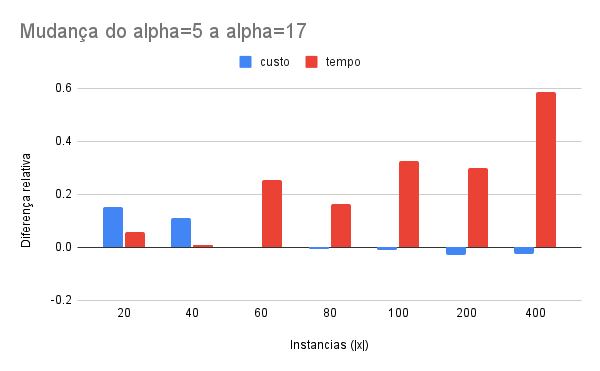
\includegraphics[width=\linewidth]{alpha17.png}\par
    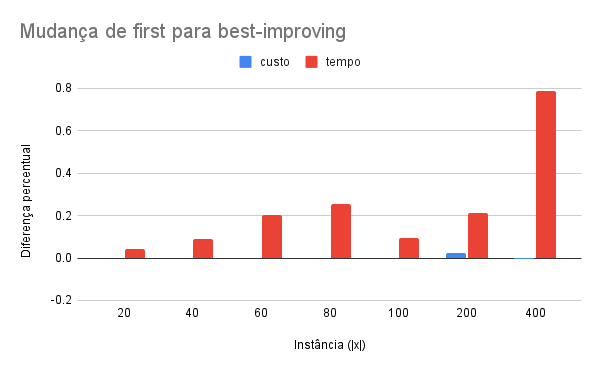
\includegraphics[width=\linewidth]{best.png}\par
    \end{multicols}
\begin{multicols}{2}
    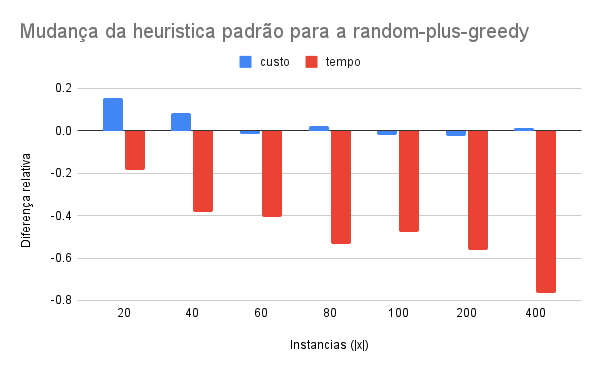
\includegraphics[width=\linewidth]{random-plus.png}\par
    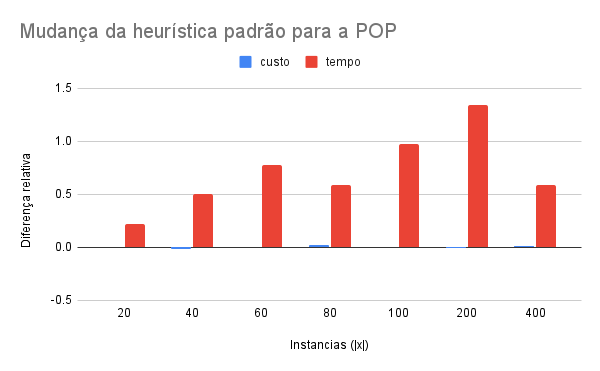
\includegraphics[width=\linewidth]{pop.png}\par
\end{multicols}
\caption{Gráficos relativos comparando as configurações [2-5] com a configuração padrão. Em azul as diferenças de custo (quanto maior, melhor) e em vermelho as diferenças de tempo em segundos (quanto menor, melhor).}
\label{graficos}
\end{figure*}

A grande diferença se mostra comparando o tempo de execução. Todas as alterações se mostraram pior no tempo que a configuração original com exceção da \emph{random-plus-greedy}, cuja melhora no tempo significativa não veio a custo de piora na solução. Ainda sobre essa métrica, é importante salientar que a instância de \(400\) variáveis na configuração \(5\) foi a única a atingir o tempo limite de \(30\) minutos, o que faria da última coluna do seu gráfico ainda maior.


Em mãos desses resultados, achamos interessante aprofundarmos na heurística \emph{random-plus-greedy}, experimentando com diferentes valores para \(p\), como demonstrado na Figura \ref{graficos_p}. Interessantemente, observamos que o valor de \(p\) relativo ao tamanho da instância não aparenta fazer tanta diferença nos valores testados, sendo consistentemente melhor que a configuração padrão em tempo e mantendo o nível de solução. Mais uma vez, acreditamos que isso se dá ao alto número de interações comparado ao baixo número de variáveis.

\begin{figure*}
\begin{multicols}{2}
    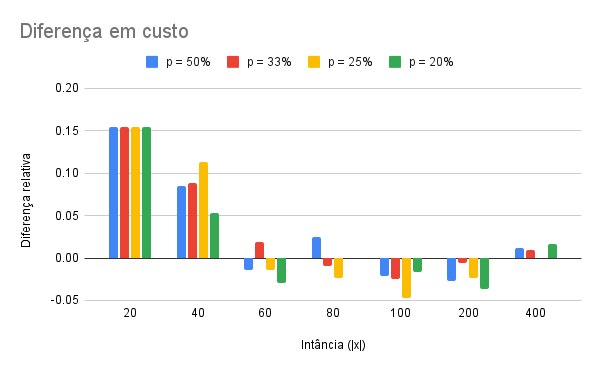
\includegraphics[width=\linewidth]{custo.png}\par
    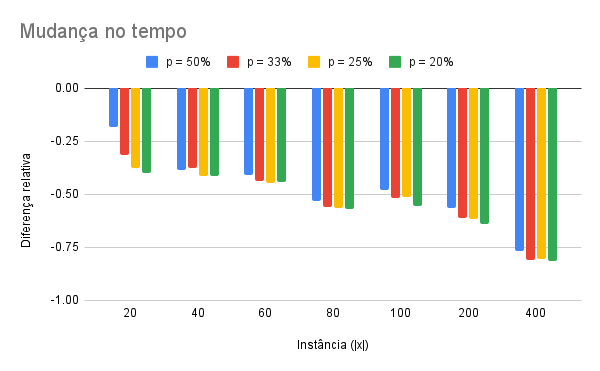
\includegraphics[width=\linewidth]{tempo.png}\par
    \end{multicols}
\caption{Gráficos relativos comparando as configurações de diferentes valores de $p$ para a heurística random-plus-greedy com a configuração padrão. A direita as diferenças de custo, a esquerda as diferenças de tempo.}
\label{graficos_p}
\end{figure*}

\printbibliography
\end{document}
